\documentclass[tikz, border=0mm]{standalone}
\usetikzlibrary{calc}
\newcommand{\tikzsetnextfilename}[1]{}


% ICON SPEC:
% - Canvas: 2x2 units, internal safe zone ~1.6x1.6
% - Colors: iconblue (RGB 70,140,255), black
% - Line width: 1.2mm base via [icon]
% - All icons must compile standalone
% - SVG export: dvisvgm --no-fonts --exact


% Global style for icons
\tikzset{
  icon/.style={
    line width=1.2mm,
    line cap=round,
    line join=round
  },
  icon-outline/.style={
    icon,
    draw=black
  },
  icon-fill/.style={
    icon,
    draw=black,
    fill=blue!60
  },
  thinner/.style={line width=0.7mm},
  thick/.style={line width=2mm},
  node-dot/.style={circle, fill=black, minimum size=4pt, inner sep=0pt},
  node-blue/.style={circle,line width=0.7mm, fill=iconblue, draw=black, minimum size=6pt, inner sep=0pt},
  node-black/.style={circle,line width=0.7mm, fill=black, draw=black, minimum size=6pt, inner sep=0pt}
}


\definecolor{iconblue}{RGB}{70,140,255}
\definecolor{iconblack}{RGB}{0,0,0}
\definecolor{iconlight}{RGB}{245,247,249}

% REUSABLE COMMANDS
\newcommand{\cardframe}{
  \useasboundingbox (-1,-1) rectangle (1,1);
  \draw[rounded corners=0.25cm] (-0.9,-0.9) rectangle (0.9,0.9);
}


\newcommand{\iconvshift}{0.07cm}
\newcommand{\iconvcenter}[1]{%
  \begin{scope}[yshift=\iconvshift]#1\end{scope}%
}


\begin{document}

\tikzsetnextfilename{card-preliminaries}

\begin{tikzpicture}[icon]
  \cardframe
  % bottom step (blue)
  \filldraw[iconblue,draw=black,rounded corners=0.18cm]
    (-0.55,-0.7) rectangle (0.75,-0.3);
  % middle step
  \draw[black,rounded corners=0.18cm]
    (-0.55,-0.15) rectangle (0.35,0.25);
  % top step
   \draw[black,rounded corners=0.18cm]
    (-0.55,0.4) rectangle (-0.05,0.8);
\end{tikzpicture}

\tikzsetnextfilename{card-permutationMatrix}
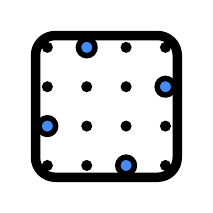
\begin{tikzpicture}[icon]
  \cardframe
  % 4x4 lattice of small dots
  \foreach \i in {0,...,3} {
    \foreach \j in {0,...,3} {
      \node[node-dot] at (-0.75 + 0.5*\i, -0.75 + 0.5*\j) {};
    }
  }
  % permutation matrix dots: permutation (2,4,1,3)
  \foreach \x/\y in {1/2, 2/4, 3/1, 4/3} {
    \pgfmathsetmacro{\xx}{-0.75 + 0.5*(\x-1)}
    \pgfmathsetmacro{\yy}{-0.75 + 0.5*(\y-1)}
    \node[node-blue] at (\xx,\yy) {};
  }
\end{tikzpicture}

\tikzsetnextfilename{card-q-analogs}

\begin{tikzpicture}[icon]
  \cardframe

  \begin{scope}[shift={(-0.6,-0.6)}]

    \draw[gray!50, line width=1.5pt, rounded corners=2pt] (0,0) rectangle (1.2,1.2);
    \foreach \x/\y in {0/0, 1/0, 0/1} {
       \fill[iconblue] (\x*0.4, \y*0.4) rectangle ++(0.4, 0.4);
       % Individual cell borders for clarity
       \draw[black, line width=1pt] (\x*0.4, \y*0.4) rectangle ++(0.4, 0.4);
    }
    \draw[black] (0, 1.2) -- (0, 0.8) -- (0.4, 0.8) -- (0.4, 0.4) -- (0.8, 0.4) -- (0.8, 0) -- (1.2, 0);

    \fill[black] (0, 1.2) circle (0.08);
    \fill[black] (1.2, 0) circle (0.08);
  \end{scope}
\end{tikzpicture}


\tikzsetnextfilename{card-representationTheory}
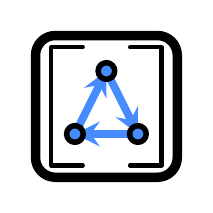
\begin{tikzpicture}[icon]
  \cardframe
  % Matrix brackets
  \draw[line width=1.5pt]
    (-0.3, 0.75) -- (-0.7, 0.75) -- (-0.7, -0.75) -- (-0.3, -0.75)
    (0.3, 0.75) -- (0.7, 0.75) -- (0.7, -0.75) -- (0.3, -0.75);
  % Three dots in a triangle
  \coordinate (A) at (0, 0.45);
  \coordinate (B) at (-0.4, -0.35);
  \coordinate (C) at (0.4, -0.35);
  % Cycling arrows (Blue)
  \draw[iconblue, ->, >=stealth, line width=1mm] (A) -- (C);
  \draw[iconblue, ->, >=stealth, line width=1mm] (C) -- (B);
  \draw[iconblue, ->, >=stealth, line width=1mm] (B) -- (A);
  % Basis Nodes
  \node[node-blue] at (A) {};
  \node[node-blue] at (B) {};
  \node[node-blue] at (C) {};

\end{tikzpicture}

\tikzsetnextfilename{card-lagrangeInversion}

\begin{tikzpicture}[icon]
  \cardframe
  % outer circle
  \draw (0,0) circle (0.70);
  % nested arcs
  \draw (-0.50,0.15) arc (180:0:0.50);
  \draw (-0.35,0.35) arc (180:0:0.35);
  % inner blue disc at bottom
  \filldraw[iconblue] (0,-0.35) circle (0.22);
\end{tikzpicture}

\tikzsetnextfilename{card-lgvLemma}
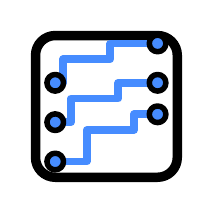
\begin{tikzpicture}[icon]
  \cardframe
  \tikzset{lgvpath/.style={line width=2.8pt,draw=iconblue}}
  % Path 1 (bottom)
  \draw[lgvpath]
    (-0.65,-0.7) -- (-0.25,-0.7) -- (-0.25,-0.3)
    -- (0.35,-0.3) -- (0.35,-0.1) -- (0.65,-0.1);
  % Path 2 (middle)
  \draw[lgvpath]
    (-0.65,-0.2) -- (-0.45,-0.2) -- (-0.45,0.1)
    -- (0.15,0.1) -- (0.15,0.3) -- (0.65,0.3);
  % Path 3 (top)
  \draw[lgvpath]
    (-0.65,0.3) -- (-0.55,0.3) -- (-0.55,0.6)
    -- (0.05,0.6) -- (0.05,0.8) -- (0.65,0.8);
  % starting points
  \foreach \y in {-0.7,-0.2,0.3}{
    \node[node-blue] at (-0.65,\y) {};
  }
  % endpoints
  \foreach \y in {-0.1,0.3,0.8}{
    \node[node-blue] at (0.65,\y) {};
  }
\end{tikzpicture}

\tikzsetnextfilename{card-polynomialIndex}

\begin{tikzpicture}[icon]
  \cardframe
  % three stacked database cylinders
  \foreach \shift/\col in {-0.15/iconblue, 0.25/iconblue, 0.55/iconblue} {
    \begin{scope}[yshift=\shift cm]
      % cylinder body
      \fill[\col]
        (-0.7,0) -- (-0.7,-0.35)
        arc (-180:0:0.7 and 0.22)
        -- (0.7,0)
        arc (0:180:0.7 and 0.22);
      \draw (-0.7,0) -- (-0.7,-0.35) arc (-180:0:0.7 and 0.22) -- (0.7,0);
      % top ellipse
      \draw (-0.7,0) arc (180:360:0.7 and 0.22);
      \draw[densely dotted] (0.7,0) arc (0:180:0.7 and 0.22);
    \end{scope}
  }
\end{tikzpicture}

\tikzsetnextfilename{card-plethysm}

\begin{tikzpicture}[icon]
  \cardframe
  % Outer Container (Function f)
  \draw[black,thinner] (-0.6, -0.6) rectangle (0.6, 0.6);
  % Inner Object (Function g)
  \filldraw[iconblue, draw=black] (0,0) circle (0.25);
  % Composition arrows
  \draw[->, >=stealth, black, thinner] (-0.5, 0.5) -- (-0.2, 0.2);
  \draw[->, >=stealth, black, thinner] (0.5, -0.5) -- (0.2, -0.2);
\end{tikzpicture}

\tikzsetnextfilename{card-schurPositivity}

\begin{tikzpicture}[icon]
  \cardframe
  % Diamond
  \filldraw[iconblue, draw=black] (0, 0.7) -- (0.7, 0) -- (0, -0.7) -- (-0.7, 0) -- cycle;
  % White plus sign
  \draw[white, thinner, line cap=round] (0, -0.35) -- (0, 0.35);
  \draw[white, thinner, line cap=round] (-0.35, 0) -- (0.35, 0);
\end{tikzpicture}

\tikzsetnextfilename{card-diagonalHarmonics}

\begin{tikzpicture}[icon]
  \cardframe
  % Nabla Symbol (inverted triangle)
  \filldraw[iconblue, draw=black]
    (-0.65, 0.55) -- (0.65, 0.55) -- (0, -0.65) -- cycle;
\end{tikzpicture}

\tikzsetnextfilename{card-latticeModel}
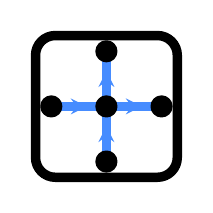
\begin{tikzpicture}[icon]
  \cardframe

  % Six-Vertex Model (Ice Rule: 2 in, 2 out)
  \coordinate (Center) at (0,0);
  \coordinate (N) at (0, 0.7);
  \coordinate (S) at (0, -0.7);
  \coordinate (W) at (-0.7, 0);
  \coordinate (E) at (0.7, 0);

  % Edge segments (full lines)
  % These establish the path lines and should be drawn first
  \draw[iconblue] (W) -- (Center);
  \draw[iconblue] (S) -- (Center);
  \draw[iconblue] (Center) -- (N);
  \draw[iconblue] (Center) -- (E);

  % West → Center (Incoming)
  % Midpoint is -0.35. Draw from -0.45 to -0.25.
  \draw[iconblue, ->, >=stealth, line width=1.5pt] (-0.45, 0) -- (-0.25, 0);

  % South → Center (Incoming)
  % Midpoint is -0.35. Draw from y=-0.45 to y=-0.25.
  \draw[iconblue, ->, >=stealth, line width=1.5pt] (0, -0.45) -- (0, -0.25);

  % Center → North (Outgoing)
  % Midpoint is 0.35. Draw from y=0.25 to y=0.45.
  \draw[iconblue, ->, >=stealth, line width=1.5pt] (0, 0.25) -- (0, 0.45);

  % Center → East (Outgoing)
  % Midpoint is 0.35. Draw from x=0.25 to x=0.45.
  \draw[iconblue, ->, >=stealth, line width=1.5pt] (0.25, 0) -- (0.45, 0);
  % Vertices (Drawn on top)
  \node[node-black] at (Center) {};
  \node[node-black] at (N) {};
  \node[node-black] at (S) {};
  \node[node-black] at (E) {};
  \node[node-black] at (W) {};

\end{tikzpicture}


\tikzsetnextfilename{card-rsk}
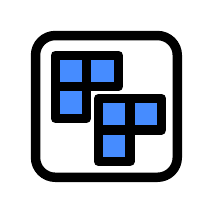
\begin{tikzpicture}[icon]
  \cardframe
  % Tableau P (Background)
  \begin{scope}[shift={(-0.65, 0.65)}]
    \fill[iconblue] (0,0) -- (0.8,0) -- (0.8,-0.4) -- (0.4,-0.4) -- (0.4,-0.8) -- (0,-0.8) -- cycle;
    \draw (0,0) rectangle (0.4,-0.4);
    \draw (0.4,0) rectangle (0.8,-0.4);
    \draw (0,-0.4) rectangle (0.4,-0.8);
  \end{scope}
  % Tableau Q (Foreground)
  \begin{scope}[shift={(-0.1, 0.1)}]
    \fill[iconblue] (0,0) -- (0.8,0) -- (0.8,-0.4) -- (0.4,-0.4) -- (0.4,-0.8) -- (0,-0.8) -- cycle;
    \draw (0,0) rectangle (0.4,-0.4);
    \draw (0.4,0) rectangle (0.8,-0.4);
    \draw (0,-0.4) rectangle (0.4,-0.8);
  \end{scope}
\end{tikzpicture}

\tikzsetnextfilename{card-root-systems}
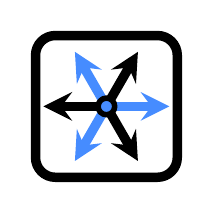
\begin{tikzpicture}[icon]
  \cardframe
  % Hexagonal Root System (A2)
  \foreach \ang in {0,120,240} {
    \draw[iconblue, ->, >=stealth, line width=1.2mm] (0,0) -- (\ang:0.8);
  }
  \foreach \ang in {60,180,300} {
    \draw[->, >=stealth, line width=1.2mm] (0,0) -- (\ang:0.8);
  }
  \node[node-blue] at (0,0) {};
\end{tikzpicture}

\tikzsetnextfilename{card-crystals}
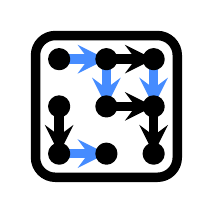
\begin{tikzpicture}[icon]
  \cardframe

  \coordinate (P11) at (-0.6, 0.6); \coordinate (P12) at (0, 0.6);    \coordinate (P13) at (0.6, 0.6);
  \coordinate (P21) at (-0.6, 0);   \coordinate (P22) at (0, 0);      \coordinate (P23) at (0.6, 0);
  \coordinate (P31) at (-0.6, -0.6);\coordinate (P32) at (0, -0.6);   \coordinate (P33) at (0.6, -0.6);
  % Blue edges (label 1)
  \draw[iconblue, ->, >=stealth] (P11) -- (P12);
  \draw[iconblue, ->, >=stealth] (P12) -- (P22);
  \draw[iconblue, ->, >=stealth] (P13) -- (P23);
  \draw[iconblue, ->, >=stealth] (P31) -- (P32);
  % Black edges (label 2)
  \draw[black, ->, >=stealth] (P12) -- (P13);
  \draw[black, ->, >=stealth] (P21) -- (P31);
  \draw[black, ->, >=stealth] (P22) -- (P23);
  \draw[black, ->, >=stealth] (P23) -- (P33);
  % Nodes
  \foreach \r in {0.6, 0, -0.6} {
    \foreach \c in {-0.6, 0, 0.6} {
      \node[node-black] at (\c, \r) {};
    }
  }
\end{tikzpicture}

\tikzsetnextfilename{card-tableau-operations}

\begin{tikzpicture}[icon]
  \cardframe
  \def\b{0.55}
  \coordinate (Origin) at (-0.7, 0.1);
  % Fixed boxes
  \draw[black] (Origin) rectangle ++(\b, \b);
  \draw[black] ($(Origin)+(\b,0)$) rectangle ++(\b, \b);
  \draw[black] ($(Origin)+(0,-\b)$) rectangle ++(\b, \b);
  % Sliding box
  \coordinate (Slider) at ($(Origin)+(\b,-\b) + (0.35, 0)$);
  \filldraw[iconblue, draw=black] (Slider) rectangle ++(\b, \b);
\end{tikzpicture}

\tikzsetnextfilename{card-cyclicSieving}
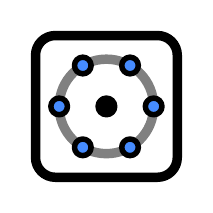
\begin{tikzpicture}[icon]
  \cardframe
  \def\rad{0.6}
  % Orbit circle
  \draw[gray] (0,0) circle (\rad);
  % 6 orbit points
  \foreach \i in {0,60,...,300} {
   \node[node-blue] at (\i:\rad) {};
  }
  \node[node-black] at (0,0) {};
\end{tikzpicture}

\tikzsetnextfilename{card-cspWord}
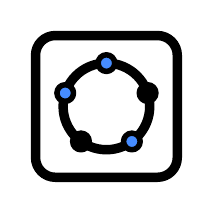
\begin{tikzpicture}[icon]
  \cardframe
  % Necklace (Circular Word)
  \def\rad{0.55}
  \draw[black] (0,0) circle (\rad);
  % Beads (Pattern: Blue, Blue, White, Blue, White)
  \node[node-blue] at (90:\rad) {};
  \node[node-blue] at (162:\rad) {};
  \node[node-black] at (234:\rad) {};
  \node[node-blue] at (306:\rad) {};
  \node[node-black] at (18:\rad) {};
\end{tikzpicture}

\tikzsetnextfilename{card-cspPath}

\begin{tikzpicture}[icon]
  \cardframe
  % Lattice Path in a box
  \draw[gray!50, line width=1pt] (-0.6,-0.6) rectangle (0.6,0.6);
  % The path
  \draw[iconblue]
    (-0.6,-0.6) -- (-0.6,-0.2) -- (-0.2,-0.2) -- (-0.2,0.2) -- (0.6,0.2) -- (0.6,0.6);
  % Start/End dots
    \node[node-black] at (-0.6,-0.6) {};
    \node[node-black] at (0.6,0.6) {};
\end{tikzpicture}

\tikzsetnextfilename{card-cspCatalan}

\begin{tikzpicture}[icon]
  \cardframe
  % Polygon Triangulation (Hexagon)
  \def\rad{0.65}
  \coordinate (A) at (90:\rad);
  \coordinate (B) at (150:\rad);
  \coordinate (C) at (210:\rad);
  \coordinate (D) at (270:\rad);
  \coordinate (E) at (330:\rad);
  \coordinate (F) at (30:\rad);
  % Polygon outline
  \draw[black] (A)--(B)--(C)--(D)--(E)--(F)--cycle;
  % Non-crossing diagonals
  \draw[black] (A) -- (C);
  \draw[black] (A) -- (D);
  \draw[black] (A) -- (E);
  % Highlight one triangle
  \fill[iconblue, opacity=1] (A)--(E)--(F)--cycle;
  \draw[black] (A)--(E)--(F)--cycle;
\end{tikzpicture}

\tikzsetnextfilename{card-cspMatch}
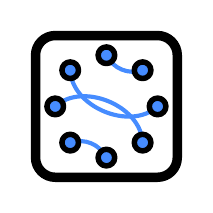
\begin{tikzpicture}[icon]
  \cardframe
  \def\rad{0.65}
  % Define coordinates
  \foreach \i in {0,45,...,315} {
    \coordinate (P\i) at (\i:\rad);
  }
  % Draw matchings
  \draw[iconblue, line width=1.5pt] (P45) to[bend left=40] (P90);
  \draw[iconblue, line width=1.5pt] (P0) to[bend left=65] (P135);
  \draw[iconblue, line width=1.5pt] (P225) to[bend left=40] (P270);
  \draw[iconblue, line width=1.5pt] (P180) to[bend left=65] (P315);
  % Draw vertices on top
  \foreach \i in {0,45,...,315} {
    \node[node-blue] at (P\i) {};
  }
\end{tikzpicture}

\tikzsetnextfilename{card-cspTableau}
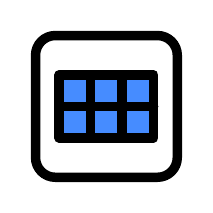
\begin{tikzpicture}[icon]
  \cardframe
  % Rectangular Young Diagram (3x2)
  \begin{scope}[shift={(-0.6, -0.4)}]
    \fill[iconblue] (0,0) rectangle (1.2, 0.8);
    \draw[black] (0,0) rectangle (1.2, 0.8);
    % Grid lines
    \draw[black] (0.4, 0) -- (0.4, 0.8);
    \draw[black] (0.8, 0) -- (0.8, 0.8);
    \draw[black] (0, 0.4) -- (1.2, 0.4);
  \end{scope}
\end{tikzpicture}

\tikzsetnextfilename{card-cspMisc}
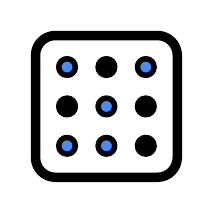
\begin{tikzpicture}[icon]
  \cardframe
  % Binary Matrix (3x3)
  \def\s{0.5}
  % Row 1
  \node[node-blue]  at (-\s,  \s) {};
  \node[node-black] at ( 0,   \s) {};
  \node[node-blue]  at ( \s,  \s) {};
  % Row 2
  \node[node-black] at (-\s,  0)  {};
  \node[node-blue]  at ( 0,   0)  {};
  \node[node-black] at ( \s,  0)  {};
  % Row 3
  \node[node-blue]  at (-\s, -\s) {};
  \node[node-blue]  at ( 0,  -\s) {};
  \node[node-black] at ( \s, -\s) {};
\end{tikzpicture}

\tikzsetnextfilename{card-gtpatterns}
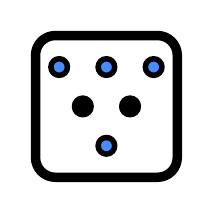
\begin{tikzpicture}[icon]
  \cardframe
  % Top row (3 dots)
  \foreach \x in {-0.6, 0, 0.6}
    \node[node-blue] at (\x, 0.5) {};
  % Middle row (2 dots)
  \foreach \x in {-0.3, 0.3}
      \node[node-black] at (\x, 0) {};
  % Bottom row (1 dot)
  \node[node-blue] at (0, -0.5) {};
\end{tikzpicture}

\tikzsetnextfilename{card-planePartitions}
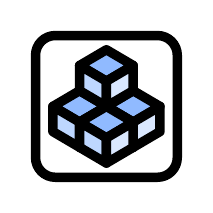
\begin{tikzpicture}[icon]
  \cardframe
  % --- isometric basis vectors (front corner view, slightly smaller) ---
  % eX: goes back-right, eY: goes back-left, eZ: goes up
  \coordinate (O)  at (0,-0.40);   % front bottom corner of the lowest cube
  \coordinate (eX) at (0.34,0.20);
  \coordinate (eY) at (-0.34,0.20);
  \coordinate (eZ) at (0,0.32);
  \coordinate (dz) at (0,-0.32);   % vertical drop to bottom faces

  % --- one cube at integer coordinates (i,j,k) ---
  \newcommand{\ppcube}[3]{%
    % top front corner of the cube
    \coordinate (T) at ($ (O) + #1*(eX) + #2*(eY) + #3*(eZ) $);
    % top face corners
    \coordinate (A) at (T);
    \coordinate (B) at ($ (T) + (eX) $);
    \coordinate (D) at ($ (T) + (eY) $);
    \coordinate (C) at ($ (B) + (eY) $);
    % bottom face corners (shifted down)
    \coordinate (Ab) at ($ (A) + (dz) $);
    \coordinate (Bb) at ($ (B) + (dz) $);
    \coordinate (Cb) at ($ (C) + (dz) $);
    \coordinate (Db) at ($ (D) + (dz) $);

    % top face (brightest)
    \path[fill=iconblue!60,draw=black]
      (A) -- (B) -- (C) -- (D) -- cycle;
    % left face
    \path[fill=iconblue!35,draw=black]
      (A) -- (D) -- (Db) -- (Ab) -- cycle;
    % right face
    \path[fill=iconblue!20,draw=black]
      (A) -- (B) -- (Bb) -- (Ab) -- cycle;
  }

  \begin{scope}
    % Bottom layer (k = 0), farthest cubes first
    \ppcube{1}{1}{0}
    \ppcube{1}{0}{0}
    \ppcube{0}{1}{0}
    \ppcube{0}{0}{0}

    % Top layer: tallest stack in the back corner
    \ppcube{1}{1}{1}
  \end{scope}
\end{tikzpicture}


\tikzsetnextfilename{card-matroid}
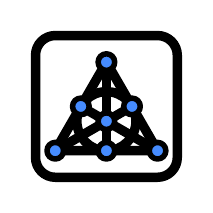
\begin{tikzpicture}[icon]
  \cardframe

  \begin{scope}[yshift=-0.1875cm]
    % Fano Plane Geometry
    \coordinate (A) at (90:0.75);
    \coordinate (B) at (210:0.75);
    \coordinate (C) at (330:0.75);
    \coordinate (M_AB) at (150:0.375);
    \coordinate (M_BC) at (270:0.375);
    \coordinate (M_CA) at (30:0.375);
    \coordinate (Center) at (0,0);
    % Circle
    \draw[black] (0,0) circle (0.375);
    % Triangle
    \draw[black] (A) -- (B) -- (C) -- cycle;
    % Medians
    \draw[black] (A) -- (M_BC);
    \draw[black] (B) -- (M_CA);
    \draw[black] (C) -- (M_AB);
    % 7 Points
    \foreach \p in {A,B,C,M_AB,M_BC,M_CA,Center} {
      \node[node-blue] at (\p) {};
    }
  \end{scope}
\end{tikzpicture}

\tikzsetnextfilename{card-dynkinDiagram}
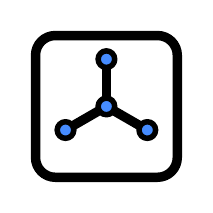
\begin{tikzpicture}[icon]
  \cardframe
  % Dynkin Diagram (D4 - Star)
  \coordinate (Center) at (0,0);
  \coordinate (N1) at (90:0.6);
  \coordinate (N2) at (210:0.6);
  \coordinate (N3) at (330:0.6);
  % Edges
  \draw[black] (Center) -- (N1);
  \draw[black] (Center) -- (N2);
  \draw[black] (Center) -- (N3);
  % Nodes
  \node[node-blue] at (Center) {};
  \node[node-blue] at (N1) {};
  \node[node-blue] at (N2) {};
  \node[node-blue] at (N3) {};

\end{tikzpicture}

\tikzsetnextfilename{card-kostantPartitionFunction}
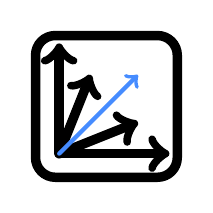
\begin{tikzpicture}[icon]
  \cardframe
  \coordinate (O) at (-0.6,-0.6);
  % Axes
  \draw[->] (O) -- (0.8,-0.6);
  \draw[->] (O) -- (-0.6,0.8);
  % Root directions
  \draw[->] (O) -- (0.4,-0.2);
  \draw[->] (O) -- (-0.2,0.4);
  % Weight vector
  \coordinate (W) at (0.4,0.4);
  \draw[->,iconblue, line width=1.5pt] (O) -- (W);
\end{tikzpicture}

\tikzsetnextfilename{card-kostkaFoulkes}
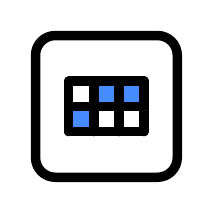
\begin{tikzpicture}[icon]
  \cardframe
  % Young diagram with charge path
  \begin{scope}[xscale=0.32,yscale=0.32,shift={(-1.5,-1)}]
    % Grid
    \foreach \x in {0,...,3}{
      \draw (\x,0) -- (\x,2);
    }
    \foreach \y in {0,...,2}{
      \draw (0,\y) -- (3,\y);
    }
    % Shape (3,2)
    \draw[line width=3pt,white] (2,1) -- (3,1) -- (2,1) -- (2,2);
    % Charge path (blue boxes)
    \fill[iconblue] (0,0) rectangle (1,1);
    \fill[iconblue] (1,1) rectangle (2,2);
    \fill[iconblue] (2,1) rectangle (3,2);
    \draw (0,0) rectangle (1,1);
    \draw (1,1) rectangle (2,2);
    \draw (2,1) rectangle (3,2);
  \end{scope}
\end{tikzpicture}


\tikzsetnextfilename{card-riggedConfigurations}
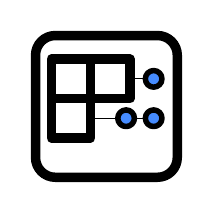
\begin{tikzpicture}[icon]
  \cardframe

  % Define Box Size
  \def\b{0.5}

  % --- The Partition (Shape) ---
  % Row 1 (Length 2)
  \filldraw[white, draw=black] (-0.7, 0.1) rectangle (-0.2, 0.6);
  \filldraw[white, draw=black] (-0.2, 0.1) rectangle (0.3, 0.6);

  % Row 2 (Length 1)
  \filldraw[white, draw=black] (-0.7, -0.4) rectangle (-0.2, 0.1);

  % --- The Riggings (Values) ---

  % Rigging for Row 1 (Value: 1 dot)
  \draw[black, thin] (0.3, 0.35) -- (0.5, 0.35); % Connector
  \node[node-blue] at (0.6, 0.35) {};

  % Rigging for Row 2 (Value: 2 dots)
  \draw[black, thin] (-0.2, -0.15) -- (0.5, -0.15); % Connector
  \node[node-blue] at (0.6, -0.15) {};
  \node[node-blue] at (0.25, -0.15) {};
\end{tikzpicture}



\tikzsetnextfilename{card-borderStripTableaux}
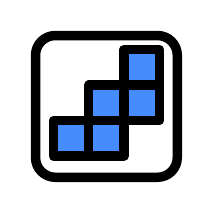
\begin{tikzpicture}[icon]
  \cardframe

  % coordinates of ribbon cells
  % (0,0), (1,0), (1,1), (2,1), (2,2)
  \begin{scope}[xscale=0.45,yscale=0.45,shift={(-1.5,-1.4)}]
    \foreach \x/\y in {0/0,1/0,1/1,2/1,2/2}{
      \path[fill=iconblue,draw=black]
        (\x,\y) rectangle ++(1,1);
    }
  \end{scope}
\end{tikzpicture}

\tikzsetnextfilename{card-littlewoodRichardsonModels}
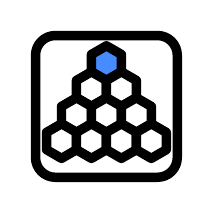
\begin{tikzpicture}[icon]
  \cardframe

  % --- Parameters ---
  \def\r{0.22}          % Hexagon radius
  \def\vsep{0.33}       % Vertical separation (1.5 * r)
  \def\hsep{0.38}       % Horizontal separation (sqrt(3) * r)

  % Calculate Vertical Centering
  % 4 rows. Top is at y_start. Bottom is y_start - 3*vsep.
  % We want the center to be 0. So y_start = 1.5 * vsep.
  \def\yStart{0.55}

  % --- Draw 1-2-3-4 Triangle ---
  \foreach \row in {1,2,3,4} {
    \foreach \col in {1,...,\row} {

      % Calculate center (cx, cy)
      % cy goes down by \vsep per row
      \pgfmathsetmacro{\cy}{\yStart - (\row-1)*\vsep}

      % cx starts offset to the left, then moves right by \hsep
      % Row 1 (1 item): 0
      % Row 2 (2 items): -0.5*hsep, 0.5*hsep
      % Formula: -(\row-1)*0.5*hsep + (\col-1)*hsep
      \pgfmathsetmacro{\cx}{-(\row-1)*0.5*\hsep + (\col-1)*\hsep}

      % Define Style: Highlight the very top hex (Row 1), others white
      \ifnum\row=1
        \def\hexstyle{iconblue}
      \else
        \def\hexstyle{white}
      \fi

      % Draw Hexagon at (cx, cy)
      \begin{scope}[shift={(\cx,\cy)}]
        \filldraw[\hexstyle, draw=black]
          (90:\r) -- (150:\r) -- (210:\r) -- (270:\r) -- (330:\r) -- (30:\r) -- cycle;
      \end{scope}
    }
  }
\end{tikzpicture}



\tikzsetnextfilename{card-polynomialRootIntro}
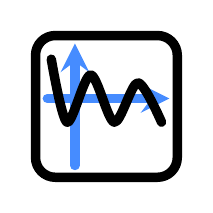
\begin{tikzpicture}[icon]
  \cardframe

  % Axes
  \draw[iconblue,-stealth] (-0.75,0.1) -- (0.8,0.1);   % x-axis
  \draw[iconblue,-stealth] (-0.4,-0.75) -- (-0.4,0.8);   % y-axis

  % A smooth polynomial curve with three x-intercepts
  \draw[black]
    plot[smooth] coordinates {
      (-0.7,0.6)
      (-0.5,-0.2)
      (-0.2,0.4)
      (0.1,-0.2)
      (0.4,0.3)
      (0.7,-0.2)
	};
\end{tikzpicture}


\tikzsetnextfilename{card-unitIntervalAO}

\begin{tikzpicture}[icon]
  \cardframe

  % Baseline (unit interval)
  \draw (-0.75,-0.5) -- (0.75,-0.5);
  \foreach \x in {-0.75,0,0.75}{
    \draw (\x,-0.55) -- (\x,-0.45);
  }

  \path[fill=iconblue,draw=black,rounded corners=2pt]
    (-0.65,-0.3) rectangle (-0.05,-0.1);
  \path[fill=iconblue,draw=black,rounded corners=2pt]
    (-0.35,0.0) rectangle (0.35,0.2);
  \path[fill=iconblue,draw=black,rounded corners=2pt]
    (0.05,0.3) rectangle (0.65,0.5);


\end{tikzpicture}



\tikzsetnextfilename{card-resources}

\begin{tikzpicture}[icon]
  \cardframe

  % 1. The Bulb (Circle + Neck)
  % We merge them visually by drawing the neck to overlap slightly

  % Glass part (Blue)
  \filldraw[iconblue, draw=black] (0, 0.2) circle (0.45);

  % Neck connection (Trapezoid, Blue to match)
  % Drawn slightly higher to cover the bottom of the circle
  \filldraw[iconblue, draw=black] (-0.25, -0.15) -- (0.25, -0.15) -- (0.2, -0.45) -- (-0.2, -0.45) -- cycle;

  % 2. The Base (Screw cap - White)
  \filldraw[iconblue, draw=black] (-0.2, -0.45) rectangle (0.2, -0.6);
  \filldraw[iconblue, draw=black] (-0.1, -0.6) rectangle (0.1, -0.7);

  % 3. The Filament (White "Spark")
  % Simple zigzag inside the blue area
  \draw[white, line width=1.5pt, line cap=round, line join=round]
    (-0.15, 0.1) -- (0, 0.35) -- (0.15, 0.1);

\end{tikzpicture}



\tikzsetnextfilename{card-personal-minor-problems}

\begin{tikzpicture}[icon]
  \cardframe

  % Little notepad / page
  \begin{scope}[xscale=0.9,yscale=0.9,shift={(-0.2,-0.1)}]
    % page outline with folded corner
    \draw[rounded corners=0.12cm]
      (-0.6,-0.6) rectangle (0.6,0.6);
    \draw (-0.6,0.3) -- (0.6,0.3); % top margin line

    \foreach \y in {0.1,-0.1,-0.3}{
      \draw[iconblue] (-0.45,\y) -- (0.45,\y);
    }
  \end{scope}

\end{tikzpicture}




\end{document}
